\chapter{Tricksters}


\begin{table*}[ht!]
\begin{small}
\rowcolors{2}{}{commentgreen}
\begin{center}
\begin{tabular}{ccccllll}
\multicolumn{5}{l}{\parbox[l][0.6cm][c]{8cm}{\textbf{The Trickster}}} & 
\multicolumn{3}{c}{\textbf{-- Spell Slots --}}
\\
\hline 
\textbf{Level} & \textbf{Prof} & \textbf{Cunning} & \textbf{Points} & \parbox[l][0.6cm][c]{8cm}{\textbf{Features}} & \textbf{1st} & \textbf{2nd} & \textbf{3rd}
\\ 
1st & +2 & 1d6 & 2 & \parbox[l][0.8cm][c]{8cm}{Expertise, \\ Thrown Weapon Fighting, Path feature} & - & - & -
\\
2nd & +2 & 1d6 & 3 & \parbox[l][0.6cm][c]{8cm}{Extra feat} & 2 & - & -
\\
3rd & +2 & 1d6 & 3 & \parbox[l][0.6cm][c]{8cm}{Path feature} & 3 & - & -
\\
4th & +2 & 1d8 & 3 & \parbox[l][0.6cm][c]{8cm}{Extra feat, Ability Score Improvement} & 3 & - & -
\\
5th & +3 & 1d8 & 4 & \parbox[l][0.6cm][c]{8cm}{Fast Movement} & 4 & 2 & -
\\
6th & +3 & 1d8 & 4 & \parbox[l][0.6cm][c]{8cm}{Extra feat} & 4 & 2 & -
\\
7th & +3 & 1d8 & 4 & \parbox[l][0.6cm][c]{8cm}{Evasion, Path feature} & 4 & 3 & -
\\
8th & +3 & 1d8 & 5 & \parbox[l][0.6cm][c]{8cm}{Extra feat, Ability Score Improvement} & 4 & 3 & -
\\
9th & +4 & 1d10 & 5 & \parbox[l][0.6cm][c]{8cm}{Path feature} & 4 & 3 & 2
\\
10th & +4 & 1d10 & 5 & \parbox[l][0.6cm][c]{8cm}{Extra feat} & 4 & 3 & 2
\\

\hline
\end{tabular}
\end{center}
\end{small}
\end{table*}




\begin{multicols*}{2}

\section*{Class Features} 

As a trickster, you gain the following class features.

\textbf{Hit Dice:} 1d8

\textbf{Hit Points at 1st Level:} 12 + your Constitution modifier

\textbf{Hit Points at Higher Levels:} 3 + your Constitution modifier per fighter level after 1st


\textbf{Armor:} Light armor, shield

\textbf{Weapons:} Simple weapons, hand crossbows, longswords, rapiers, shortswords, scimitar, longbow, whip

\textbf{Saving Throws:} Dexterity, Intelligence

\textbf{Skills:} Choose four from Acrobatics, Athletics, Deception, Insight, Intimidation, Investigation, Perception, Performance, Persuasion, Sleight of Hand, Stealth, and Survival
    
\section*{Cunning} 

You have a poll of cunning dices to use. A common use of your cunning is a strike of luck, performing an inexplicable deed. Each path specializes on the usage of cunning in a different way. For example, a bard mocks his enemies while a rogue tumbles across the battlefield.



\begin{itemize}
    \item You regain all cunning points when finish a short or long rest.
    \item Once per round, you regain 1 cunning point whenever you or an ally within sight scores a critical hit. The hit disorients the target and you chase the moment in your favor.
    \item ???;
\end{itemize}

Outside of combat, you can use a cunning die bonus to any deception, persuasion, or investigation roll. You can use cunning to cause a diversion and draw attention away from your for your cunning die minutes, e.g., a bard may shout about a muse making the public look at her while a rogue can throw a rock and draw the guard's attention to the noise while she sneaks by.

    
\section*{Expertise} 

Choose two of your skill proficiencies, or one of your skill proficiencies and your proficiency with thieves’ tools. Your proficiency bonus is doubled for any ability check you make that uses either of the chosen proficiencies.

\section*{Thrown Weapon Fighting}

Beginning at 1st level, you can draw a weapon that has the thrown property as part of the attack you make with the weapon.     In addition, when you hit with a ranged attack using a thrown weapon, you gain a +1 bonus to the damage roll.



\section*{Spellcasting}

You have learned to untangle and reshape the fabric of reality in harmony with your wishes and clever thinking.

\textbf{Cantrips}

You learn three cantrips: Mage Hand and two other cantrips of your choice. 


\textbf{Spells Known of 1st Level and Higher}

You know three 1st-level spells of your choice, two of which you must choose from the enchantment and illusion spells list.

The Trickster Spellcasting table shows how many spell slots you have to cast your spells of 1st level and higher. To cast one of these spells, you must expend a slot of the spell's level or higher. You regain all expended spell slots when you finish a long rest.


Whenever you gain a level in this class, you learn a new spell. Additionally, you can replace one of the spells you know with another spell of your choice from the trickster spell list. The new spell must be of a level for which you have spell slots.


\textbf{Spellcasting Ability}

Intelligence or Charisma is your spellcasting ability for your spells. You use your Intelligence or Charisma whenever a spell refers to your spellcasting ability. In addition, you use your Intelligence or Charisma modifier when setting the saving throw DC for a spell you cast and when making an attack roll with one.

\textbf{Spell save DC} = 8 + your proficiency bonus + your Intelligence/Charisma modifier

\textbf{Spell attack modifie}r = your proficiency bonus + your Intelligence/Charisma modifier


\section*{Fast Movement}

Starting at 5th level, your speed increases by 10 feet while you aren’t wearing heavy armor.


\section*{Evasion}

Beginning at 7th level, you can nimbly dodge out of the way of certain area effects, such as an ancient red dragon’s fiery breath or an ice storm spell. When you are subjected to an effect that allows you to make a Dexterity saving throw to take only half damage, you instead take no damage if you succeed on the saving throw, and only half damage if you fail.

    

\begin{Figure}
\centering
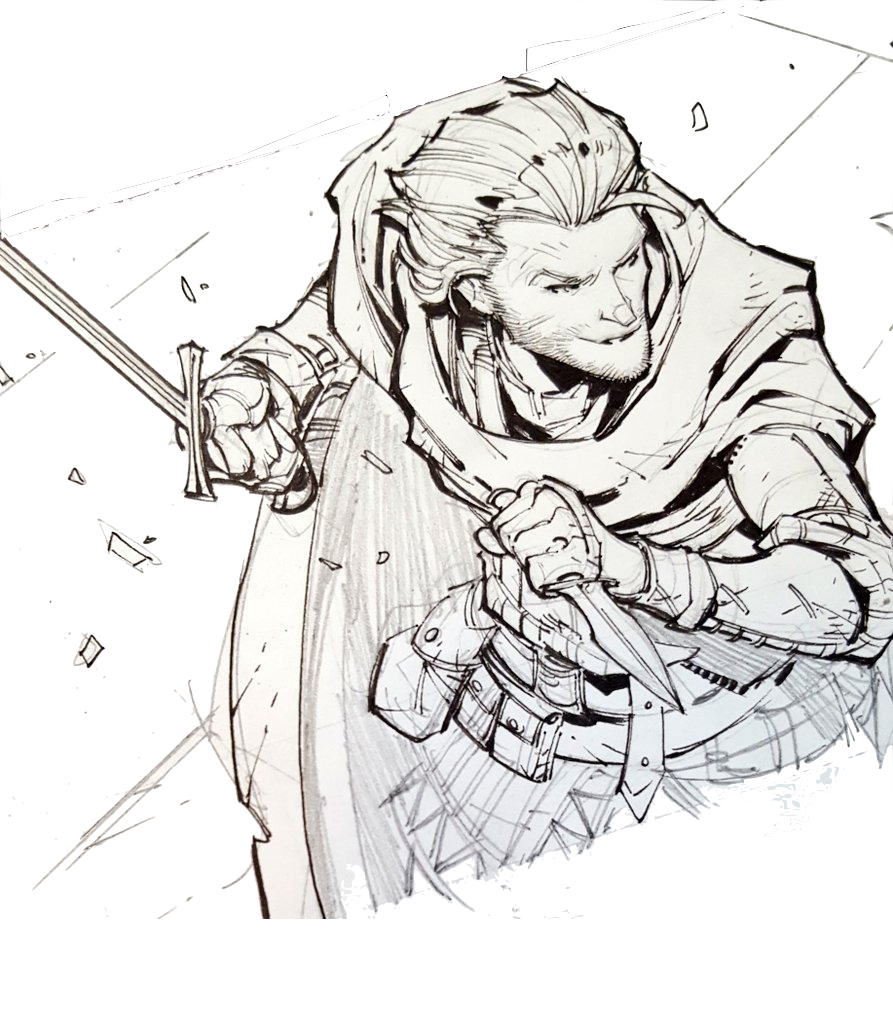
\includegraphics[width=\textwidth]{img/trickster.png}
\end{Figure}
    
\end{multicols*}

\clearpage


\begin{multicols*}{2}

\section{Bard}

\subsection*{Healing Hands}

\subsection*{Sacred Immolation}

\subsection*{Divine Smite}

\subsection*{Aura of Courage}

\begin{Figure}
\centering
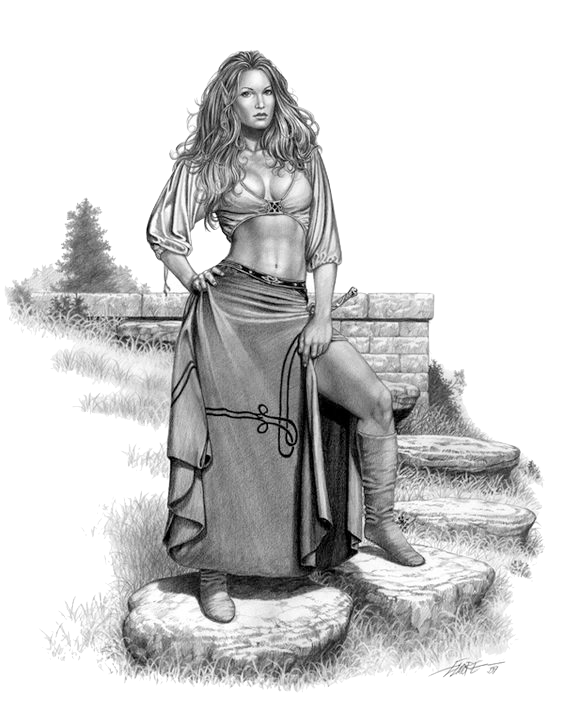
\includegraphics[width=\textwidth]{img/bard-2.png}
\end{Figure}
    
\end{multicols*}

    


\begin{multicols*}{2}

\section{Hunter}

\lettrine[lines=3, lhang=0.15, loversize=0.25, findent=.5em]{H}{unters} have undergone extensive training, ruthless mental and physical conditioning in preparation for facing all the sorts of beasts, demons, and aberrations.

\subsection*{Wanderer}

The hunter's nomadic culture allows them to adapt to the most inhospitable environments. For example, a hunter traveling through a marsh or a rain forest will quickly learn about edible and poisonous mushrooms, therefore gaining resistance to poison damage.



\begin{itemize}
    \item You have advantage on initiative rolls.
    \item You gain you proficiency with medium armor, and martial weapons.
    \item You gain resistance to either poison, cold or fire damage. Whenever you finish a long rest, you may change your damage resistance type.
    \item When you engage in two-weapon fighting, you can add your ability modifier to the damage of the second attack.    
\end{itemize}


\subsection*{Predator's Cunning}

At 3rd level, you learn maneuvers that are fueled by your cunning dice. Refer to the hunter's cunning action table for details.

\subsection*{Bird's Talons}

Starting at 5th level, you can attack twice, instead of once, whenever you take the Attack action on your turn.

If you don't have any cunning points at the start of a combat, you can burn a spell slot and have one cunning point per spell slot level instead.

\subsection*{Claw and Fang}

At 9th level, you become a legendary hunter. You gain several benefits, depending on your fighting style:

\begin{itemize}
    \item \textbf{Sword \& Shield:} When a creature hits you with an attack, you gain a +4 bonus to AC against all subsequent attacks made by that creature for the rest of the turn.
    \item \textbf{Two-weapon fighting:} You score critical-hits on 19-20
    \item \textbf{Bowmanship:} Once per turn, you can reduce the movement speed of a creature hit by your arrows by 10 feet.
\end{itemize}

\begin{Figure}
\centering
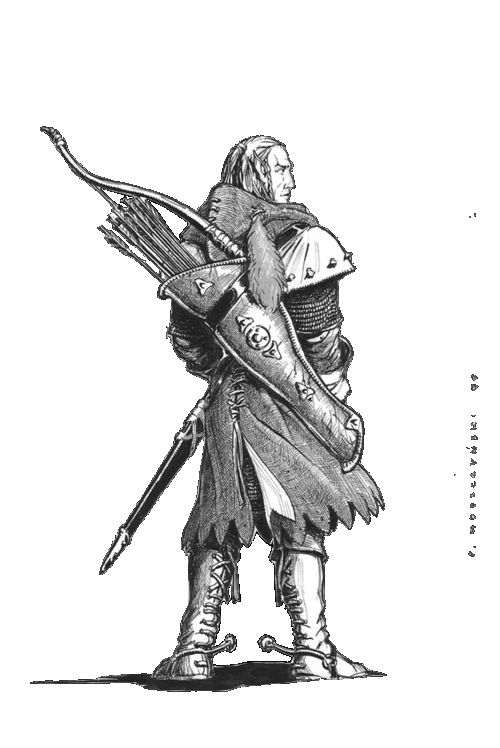
\includegraphics[width=\textwidth]{img/longbow.png}
\end{Figure}
    
\end{multicols*}


\clearpage

\begin{table}[ht!]
\begin{small}
\rowcolors{2}{}{commentgreen}
\begin{center}
\begin{tabular}{ll}
\multicolumn{2}{l}{\parbox[l][0.6cm][c]{15cm}{\textbf{Hunter Cunning Actions}}} 
\\
\hline 
\textbf{Name} & \parbox[l][0.6cm][c]{15cm}{\textbf{Description}}
\\ 
Rain of Arrows & \parbox[l][2.1cm][c]{15cm}{
As a reaction, you can spend one cunning point to make an attack of opportunity against any creature entering a space 15 feet away from you provided that you are holding a \hl{ranged} weapon.  If you hit, you add the cunning die to the attack's damage roll. Additionally, any feats or benefits applied only to melee weapons apply to your attack.
}
\\ 
Giant Killer & \parbox[l][2cm][c]{15cm}{
When a Large or larger creature within 5 feet of you hits or misses you with an attack, you can use a cunning point to spend your reaction to attack that creature immediately after its attack, provided that you can see the creature.  If you hit, you add the cunning die to the attack's damage roll.
}
\\ 
Augmenting Concoction & \parbox[l][2cm][c]{15cm}{
You can use your bonus action to 
spend one cunning point
 and drink a special potion 
that is toxic to any creature other than you. On you, 
the concotion makes you stronger. Until the end of your next turn, add your cunning die as extra damage to your attack rolls.
}
\\
Mercury Weapon & \parbox[l][2.1cm][c]{15cm}{
You can use your bonus action to 
spend one cunning point and dilute a mercury like chemical element over a pair of \hl{melee} weapons or \hl{20 missiles}. For the next 10 minutes, your weapons count as magical for the purpose of overcoming magical resistance
and receive a +1 bonus to attack and damage rolls.
}
\\
Herbal Vigor & \parbox[l][1.8cm][c]{15cm}{
You can use your bonus action to 
spend one cunning point and chew a special set or herbs to strengthen your immune system. For 1 hour, 
you gain resistance to poison damage and you gain temporary hit points equals to your cunning die.
}
\\
\hline
\end{tabular}
\end{center}
\end{small}
\end{table} 


\begin{multicols*}{2}
\begin{Figure}
\centering
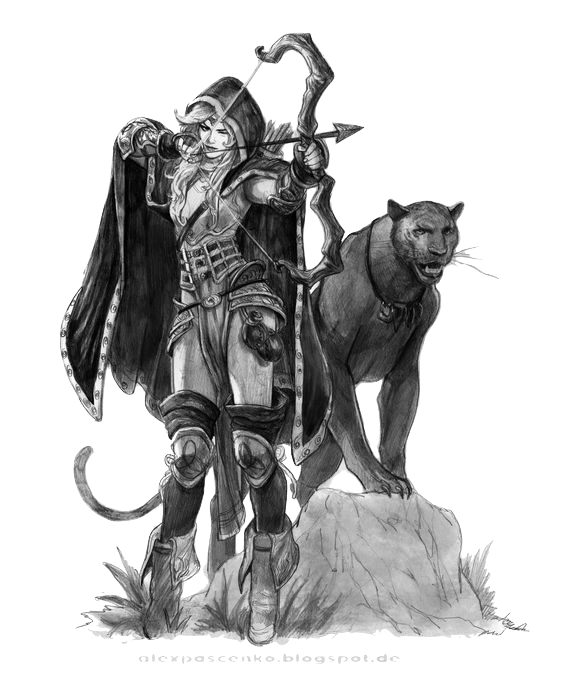
\includegraphics[width=\textwidth]{img/hunter-panther.png}
\end{Figure}
    
\end{multicols*}    


\begin{multicols*}{2}

\section{Thief}

\lettrine[lines=3, lhang=0.15, loversize=0.25, findent=.5em]{T}{hieves} are experts at stealth and surprise, they can move through the shadows, vanish into thin air, or steal items from their opponents in the blink of an eye. 

\subsection*{Sneak Attack}

Beginning at 1st level, you know how to strike subtly and exploit a foe’s distraction. Once per turn, you can deal an extra 1d6 damage to one creature you hit with an attack if you have advantage on the attack roll. The attack must use a finesse or a ranged weapon.

You don’t need advantage on the attack roll if another enemy of the target is within 5 feet of it, that enemy isn’t incapacitated, and you don’t have disadvantage on the attack roll.

The amount of the extra damage increases as you gain levels in this class, as shown in the table below.

\header{Sneak attack damage}
\begin{rpg-table}
   	\textbf{Level}  & \textbf{Sneak Attack} \\
   	1st  & 1d6 \\
   	2nd  & 1d6 \\
    3rd  & 2d6 \\
    4th  & 2d6 \\
    5th  & 3d6 \\
    6th  & 3d6 \\
    7th  & 4d6 \\
    8th  & 4d6 \\
    9th  & 5d6 \\
    10th & 5d6 \\
\end{rpg-table}




\subsection*{Cunning Action}

At 3rd level, you learn maneuvers that are fueled by your cunning dice. Refer to the rogue's cunning action table for details.

\subsection*{Etheral Jaunt}

You are a master of subterfuge. At 5th level, you can see normally in darkness, both magical and nonmagical, to a distance of 30 feet.

Additionally, you gain the ability to step from one shadow into another. When you are in dim light or darkness, as a bonus action you can teleport up to 60 feet to an unoccupied space you can see that is also in dim light or darkness. The teleport action is either of magical nature or raw physical reflexes. 

You can use this feature three times. You regain all expended uses of it when you finish a long rest. You can burn cunning point for additional uses.

\subsection*{Pierce the Veil}

Like a ghost, you have the ability to slip in and out of the Ethereal Plane.

Starting at the 9th level, you can use your cunning action in your first turn of a combat to cast the blink spell.

Once you use this feature, you can’t use it again until you finish a long rest or until you spend a spell slot of 3rd level or higher.

\begin{Figure}
\centering
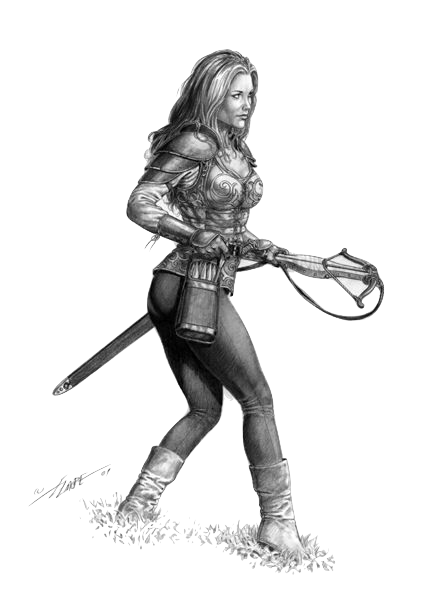
\includegraphics[width=\textwidth]{img/female-rogue.png}
{\scriptsize Art by Larry Elmore}
\end{Figure}
    
\end{multicols*}


\clearpage

\begin{table}[ht!]
\begin{small}
\rowcolors{2}{}{commentgreen}
\begin{center}
\begin{tabular}{ll}
\multicolumn{2}{l}{\parbox[l][0.6cm][c]{15cm}{\textbf{Rogue Cunning Actions}}} 
\\
\hline 
\textbf{Name} & \parbox[l][0.6cm][c]{15cm}{\textbf{Description}}
\\ 
Quick Footwork & \parbox[l][1.8cm][c]{15cm}{
Your quick thinking and agility allow you to move and act quickly. You can spend one cunning point to take a bonus action on each of your turns in combat. This action can be used only to take the Dash, Disengage, or Hide action.
}
\\ 
Quick Reflexes & \parbox[l][1.2cm][c]{15cm}{
You can spend one cunning point to take the Dodge action as a bonus action on your turn.
}
\\ 
Fast Hands & \parbox[l][1.8cm][c]{15cm}{
You can spend one cunning point and use your bonus action to make a Dexterity (Sleight of Hand) check, use your thieves' tools to disarm a trap or open a lock, or take the Use an Object action.
}
\\
Precision Attack & \parbox[l][1.8cm][c]{15cm}{
When you make a weapon attack roll against a creature, you can expend one cunning die to add it to the roll. You can use this maneuver before or after making the attack roll, but before any effects of the attack are applied.
}
\\
Slow Fall & \parbox[l][1.2cm][c]{15cm}{
You can use your reaction when you fall to spend one cunning point and reduce any falling damage you take by an amount equal to five times your cunning die.
}
\\
\hline
\end{tabular}
\end{center}
\end{small}
\end{table}    


    

